\section{Caratteristica volt-amperometrica di una lampadina}
Per eseguire l'analisi di un carico resistivo non ohmico abbiamo utilizzato come soggetto del test una lampadina. Sappiamo che, quando abbiamo davanti una resistenza che si comporta in modo ``ohmico'', il grafico della caratteristica volt-amperometrica è una retta passante per l'origine. Nel caso della lampadina, ci aspettiamo dunque una curva non lineare. Abbiamo sottoposto il circuito (identico a quello in Figura \ref{fig:circuiti}, con la lampadina al posto della resistenza Rx) a diversi valori di tensione fino a quello massimo di 12V. I risultati sono riportati nel grafico in Figura \ref{fig:lampadina}.

\begin{figure}[h]
    \centering
        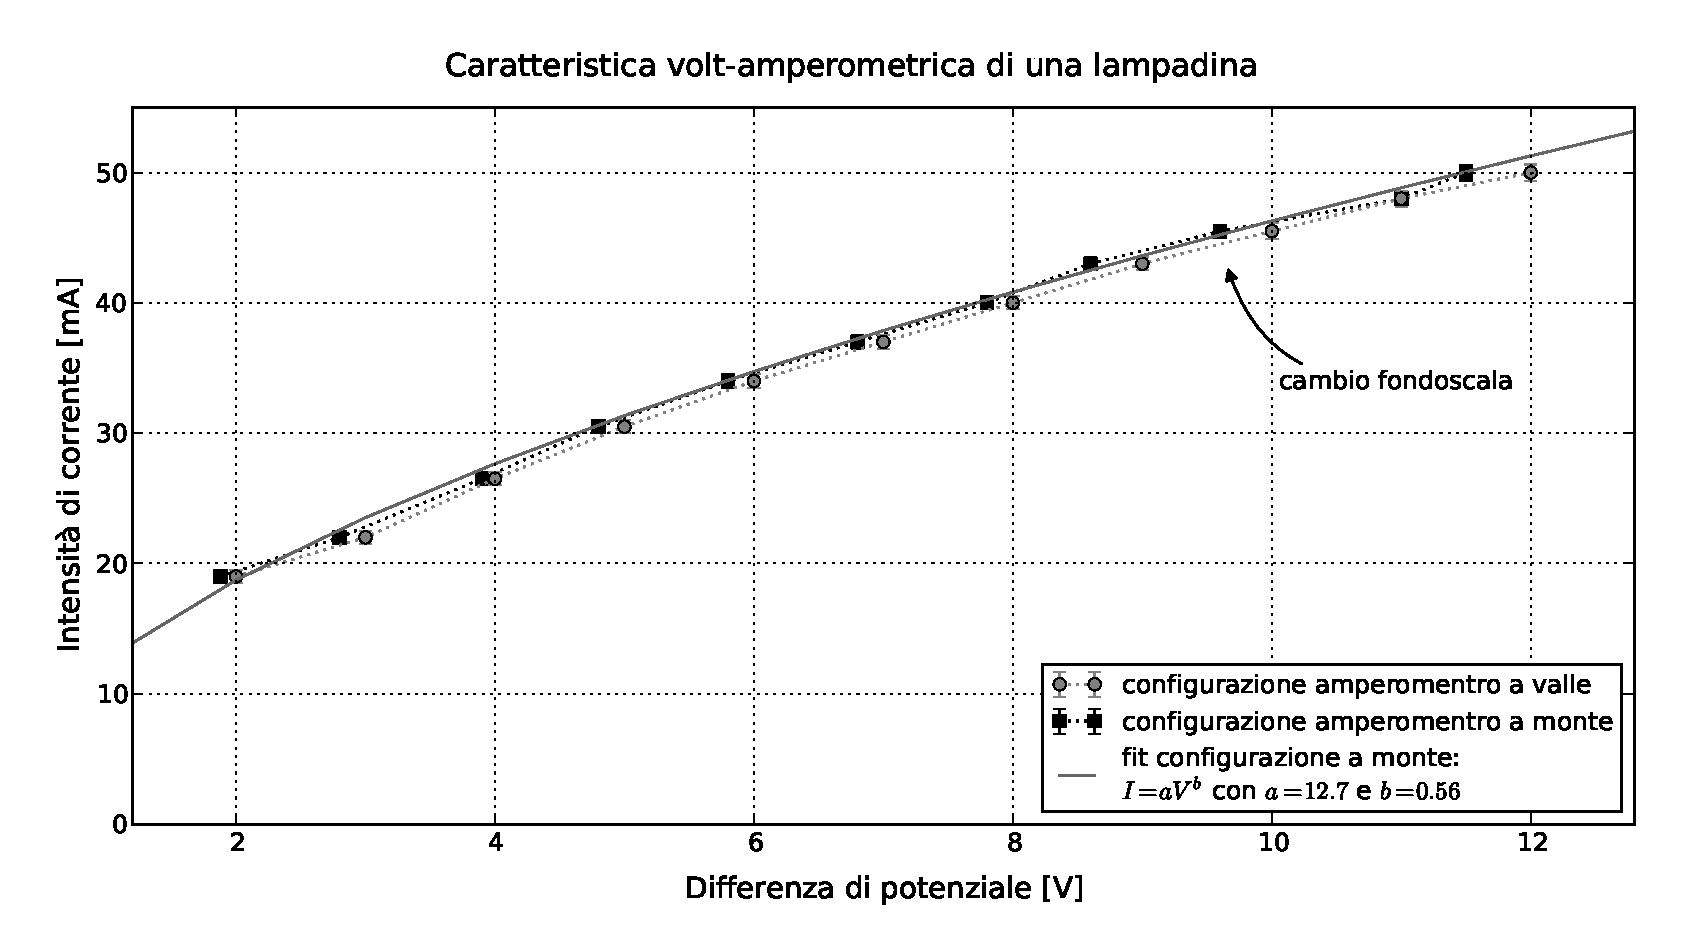
\includegraphics[width=\textwidth]{lamp.eps}
        \caption{Il grafico mostra la caratteristica volt-amperometrica di un carico resistivo non ohmico (lampadina).}
        \label{fig:lampadina}
\end{figure}

Si può notare che il circuito è sicuramente non ohmico, ma dai dati non risulta ovvia la funzione che definisce la caratteristica volt-amperomentrica della lampadina.